% Answers to the Section 3 Review Questions, book pp. 453-456 (PDF pp. 454-457).
% The answer key's own numbering, which matches the 14 printed questions.
\begin{enumerate}
\item
\begin{enumerate}
  \item[a.] $x = 3, -\frac{1}{3}, -\frac{1}{2}$
  \item[b.] $x = 1, -\frac{2}{5}, -1$
\end{enumerate}
\item
\begin{enumerate}
  \item[a.] the zeros are -1, 0.5. and 3
  \item[b.] the factors are $(x + 1)\,(2x\text{-}1)\,(x\text{-}3)$
  \item[c.] --1 $>$ x, --1 $<$ x $<$ 0.5, 0.5 $<$ x $<$ 3, x $>$ 3
  \item[d.] $f(x) = 2x^3 - 5x^2 - 4x + 3$
\end{enumerate}
\item
\begin{enumerate}
  \item[a.] \mbox{}\par\nopagebreak
  \begin{center}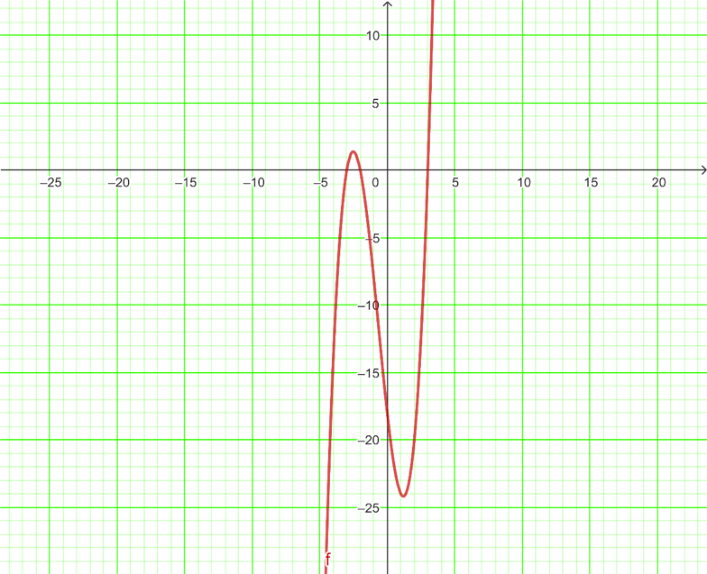
\includegraphics[width=0.55\linewidth]{figures/ans3-3a.png}\end{center}
  \item[b.] \mbox{}\par\nopagebreak
  \begin{center}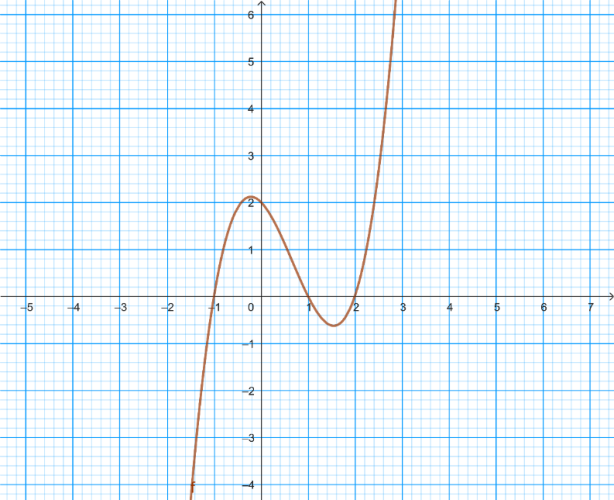
\includegraphics[width=0.55\linewidth]{figures/ans3-3b.png}\end{center}
  \item[c.] \mbox{}\par\nopagebreak
  \begin{center}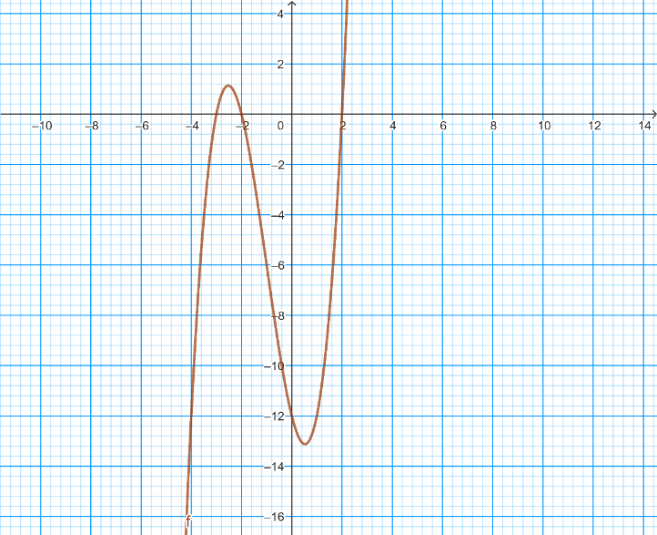
\includegraphics[width=0.55\linewidth]{figures/ans3-3c.png}\end{center}
  \item[d.] \mbox{}\par\nopagebreak
  \begin{center}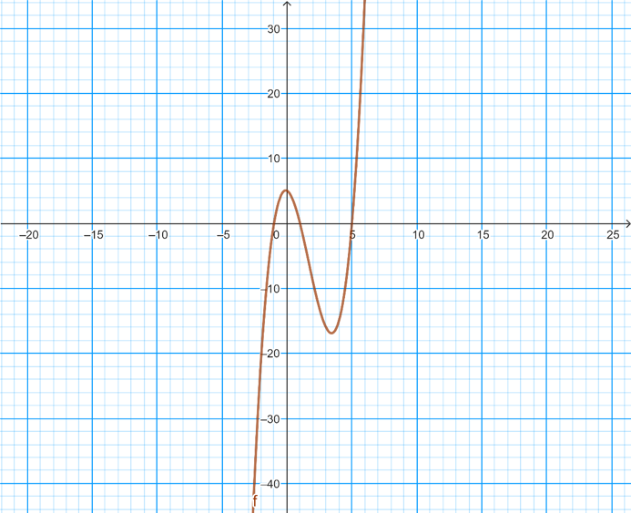
\includegraphics[width=0.55\linewidth]{figures/ans3-3d.png}\end{center}
  \item[e.] \mbox{}\par\nopagebreak
  \begin{center}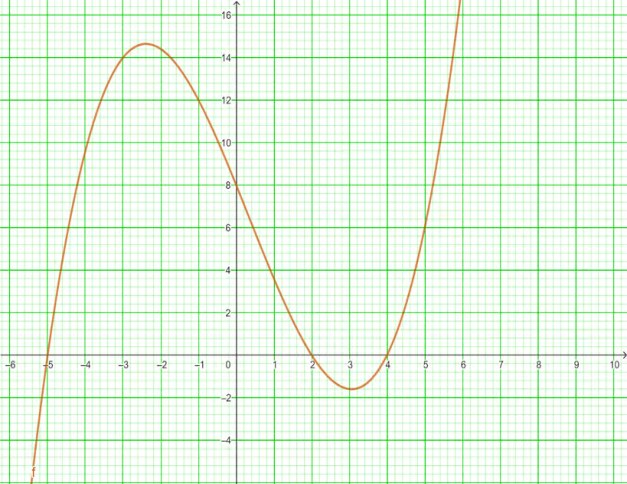
\includegraphics[width=0.55\linewidth]{figures/ans3-3e.jpg}\end{center}
\end{enumerate}
\item
\begin{enumerate}
  \item[a.] $(x - 1)(x + 2)(x + 4)$
  \item[b.] $(x + 2)(2x + 5)(x - 3)$
  \item[c.] $(x - 2)(2x -\ )(2x)$
  \booknote[S3-17]{the answer is garbled; $4x^3 - 4x^2 - 11x + 6 = (x - 2)(2x + 3)(2x - 1)$.}
  \item[d.] $(x + 2)(3x + 2)(2x - 1)$
  \item[e.] $(x - 1)(3x + 1)(x + 6)$
\end{enumerate}
\item
\begin{enumerate}
  \item[a.] $x = 1, -3, -2$
  \item[b.] $x = -5, 1, 0.5$
  \item[c.] $x = -2, 1, 0.5$
  \item[d.] $x = -1.5, 1.5, 2$
  \item[e.] $x = -0.5, 1, 0.5$
  \item[f.] $x = 1, 0.5, 1.5$
\end{enumerate}
\item
\begin{enumerate}
  \item[a.] $0, i\sqrt{6}, -i\sqrt{6}$
  \item[b.] $i\sqrt{\frac{7}{2}}, -i\sqrt{\frac{7}{2}}, -\sqrt{5}, \sqrt{5}$
  \booknote[S3-18]{$2x^4 + 17x^2 + 35 = (2x^2 + 7)(x^2 + 5)$, so the last two roots
  are $-i\sqrt{5}$ and $i\sqrt{5}$.}
  \item[c.] $-\sqrt{7 + \sqrt{13}},\ ,\ \sqrt{7 + \sqrt{13}}, -\sqrt{7 - \sqrt{13}},
  \sqrt{7 - \sqrt{13}}$
  \item[d.] $1, -1, i, -i$
  \item[e.] $0, 3i\sqrt{3}, -3i\sqrt{3}$
\end{enumerate}
\item $f(x) = x^3 - 5x^2 - 6x$
\item
\begin{enumerate}
  \item[a.] a $=$ 11, b $=$ 6
  \item[b.] $(2x + 1)(x + 2)(x + 3)$
\end{enumerate}
\booknote[S3-19]{this answer does not fit the question: $(2x + 1)(x + 2)(x + 3)
= 2x^3 + 11x^2 + 17x + 6$, whose leading coefficient is 2, not 10, and with
$a = 11$, $b = 6$ the printed $Q(x)$ gives $Q(-\frac{1}{2}) = 12.5$ and
$Q(-1) = 17$. The conditions as printed have no integer solution.}
\item $f(x) = x^4 - 6x^3 + 24x^2 - 38x + 29$
\booknote[S3-20]{$(x^2 - 2x + 3)(x^2 - 4x + 13) = x^4 - 6x^3 + 24x^2 - 38x + 39$;
the constant term should be 39.}
\item
\begin{enumerate}
  \item[a.] Positive zeros\textbf{:} 5, 3, or 1, Negative zeros\textbf{:} 0
  \item[b.] Possible Positive Zeros\textbf{:} 1, Possible Negative Zeros\textbf{:} 4, 2, or 0
  \item[c.] Possible Positive Zeros\textbf{:} 1, Possible Negative Zeros\textbf{:} 1
  \item[d.] Possible Positive Zeros\textbf{:} 0, Possible Negative Zeros\textbf{:} 2 or 0
  \item[e.] Possible Positive Zeros\textbf{:} 2 or 0, Possible Negative Zeros\textbf{:} 2 or 0
\end{enumerate}
\item
\begin{enumerate}
  \item[a.] $x^3 + 3x^2 - 13x - 15$
  \item[b.] $15x^3 - 37x^2 - 23x - 3$
  \item[c.] $x^4 - 8x^2 + 16$
  \booknote[S3-21]{$x^4 - 8x^2 + 16 = (x^2 - 4)^2$ has roots $\pm 2$ only; the
  equation with roots $2, -2, 2 \pm \sqrt{3}$ is $(x^2 - 4)(x^2 - 4x + 1) =
  x^4 - 4x^3 - 3x^2 + 16x - 4$.}
  \item[d.] $x^3 - 2x^2 + 17x$
\end{enumerate}
\item $i, -i, i\sqrt{2}, -i\sqrt{2}$
\item
\begin{enumerate}
  \item[a.] $(x + 1)(x + 2)(x + 3)(x - 1)(x - 2)$
  \item[b.] $x^5 + 3x^4 - 5x^3 - 15x^2 + 4x + 12$
  \item[c.] 4 turning points
  \item[d.] degree reduced by 1 gives the maximum number of turning points
\end{enumerate}
\item Width $=$ 20 cm, Length $=$ 24cm and Height $=$ 10 cm.
\end{enumerate}
